\chapter{User Manual}

\section{Starting up the app}
After you have installed Wattitude on your phone, as explained in chapter~\ref{sec:installWattitudePhone}, you can start using the app. 

Firstly, since this version of the app do not have support for directly connecting the app to power measuring devices in your home, you need to add data. This involves adding all the different devices you want to collect usage for and adding their usage. The usage of a device is added day by day, and if you do not know your past usage it is possible to add an average usage. This can on many devices be found on a note by the power connector on the device.

\subsection{Logging in to Facebook}
Logging in to Facebook is done by entering the "login" option in the drawer meny. This will show a login window where you need to enter your username and password. Then press the "Log In" button. 

\begin{figure}[H]
\centering
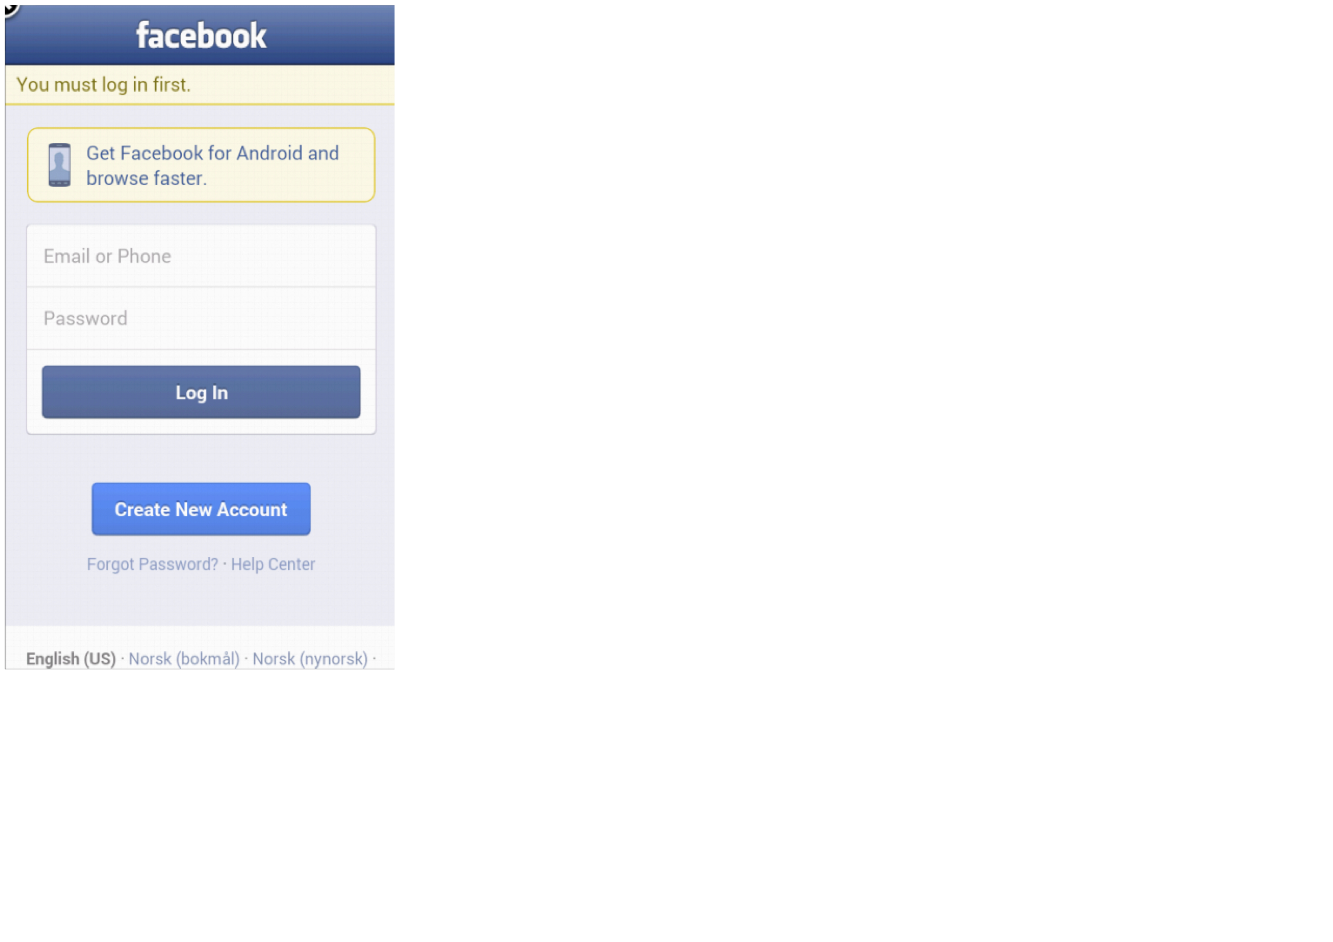
\includegraphics[width=0.9\textwidth]{appendix/usermanual/fig/Facebooklogin.png}
\caption{Screenshot of the facebook login screen}
\end{figure}


\label{sec:devices}
\section{Devices}
\subsection{Adding a new device}
To add a new device press the green plus symbol in the option menu. This will make a dialog appear, add the name of the device you want to add and what category the device falls under. It is also optional to add a description to the device.

\todo{Picture of add device dialog and the plus symbol}

\subsection{Editing a device}
To modify a device already added to your list of devices it is necessary to select the device you want to modify, by holding your finger over it. When doing this a dialog will appear. This dialog gives you the option to edit or delete the device you held in. Tap the edit button and a new dialog will appear. Enter the new values you want to save to the device you chose.

\todo{Picture of the choose dialog with edit and delete}

\subsection{Deleting a device}
To delete a device in you list of devices press the device you want to delete and select delete in the dialog that appears. A dialog asking if you really want to delete the device will show. Press OK, and you have deleted your device!

\todo{Picture of "Do you really want to delete?"}

\section{Usage}
The usage tab will give you an overview of your usage. You can see the usage of one or several devices, or you can see your total usage. Here, you can also share your usage with your Facebookfriends.
\subsection{Adding usage}
To add usage to a device, it is important to first have created a device to add usage to. This is done in the device tab. ~\ref{sec:devices}
\todo{Picture of adding usage}
\subsection{Examine your own usage}
You can examine your usage in two different ways. You can look at the usage graph in the usage tab, within the drawer menu user tab. It is also possible to look at how your consumption is distributed between all of your devices. This is done in the distribution tab, within the drawer menu usage tab. 
\todo{Add picture of the two "under tabs within the usage tab"}
\todo{Add picture of your usage, a graph screenshot}


\section{Exchange tips}
\todo{Within the exchange tips tab, you can manage all of your tips. Tips is meant to be advise that will help you save energy around your house, when completed. }

\subsection{Creating your own tip}
To create your own tip, press the green plus symbol in the option bar. This will create a dialog where you must enter a name of your new device, and a description. \todo{Er det noen restriksjoner på hva du kan skrive inn i denne dialogen? Type, må man ha beskrivelse etc.}
\subsection{Adding a tip to your list of tips}
Your list of tips is meant to be a list over the tips you want to perform in you house. To add tip to your list of tips, you select the tip you want to add and a dialog will appear. Select the "Add to my tip" option. The tip you added will now be saved in the "My tips" tab. 
\todo{Picture of my tips tab}
\todo{Picture of the add tips to my tips dialog}
\subsection{Indicate that you have performed a tip}
To indicate that you have performed a tip, you check the checkbox beside the tip.
\subsection{Rate a tip}
To change the rating of a tip you hold your finger over the tip you want to change and a dialog will appear. 

